\documentclass{standalone}
\author{Quinten Bruynseraede}
\usepackage{tikz}
\usetikzlibrary{shapes}
\title{Tikz grafen}
\begin{document}\pagestyle{empty}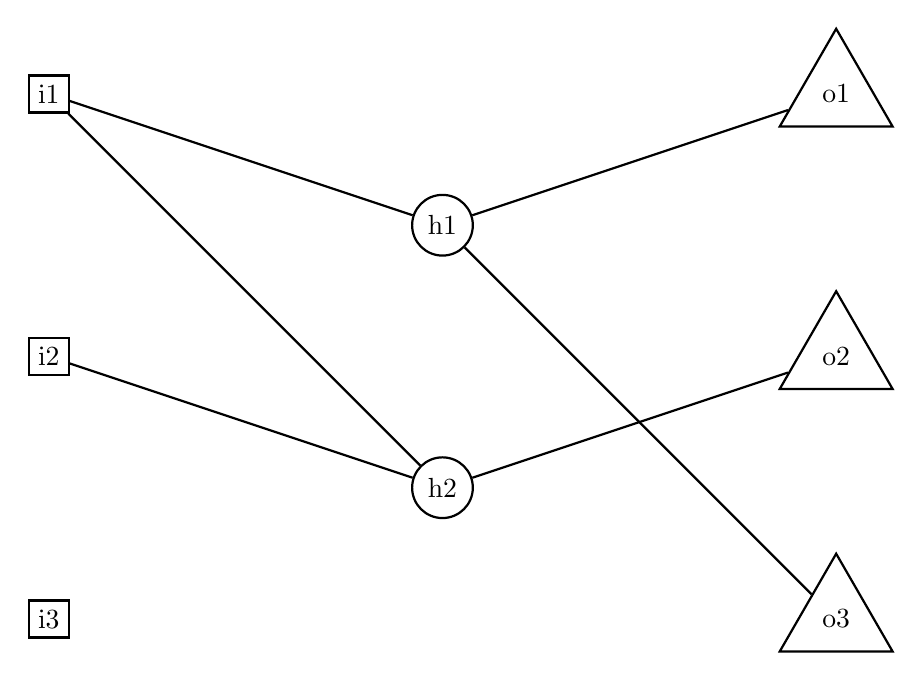
\begin{tikzpicture}\node[shape=rectangle,draw=black,align=center,line width=0.8pt] (0) at (1.6666666666666667,13.333333333333334) {i1};
\node[shape=circle,draw=black,align=center,line width=0.8pt] (1) at (6.666666666666667,11.666666666666666) {h1};
\node[shape=circle,draw=black,align=center,line width=0.8pt] (2) at (6.666666666666667,8.333333333333334) {h2};
\node[regular polygon,regular polygon sides=3,draw=black,align=center,line width=0.8pt] (3) at (11.666666666666666,13.333333333333334) {o1};
\node[regular polygon,regular polygon sides=3,draw=black,align=center,line width=0.8pt] (4) at (11.666666666666666,10.0) {o2};
\node[regular polygon,regular polygon sides=3,draw=black,align=center,line width=0.8pt] (5) at (11.666666666666666,6.666666666666667) {o3};
\node[shape=rectangle,draw=black,align=center,line width=0.8pt] (6) at (1.6666666666666667,10.0) {i2};
\node[shape=rectangle,draw=black,align=center,line width=0.8pt] (7) at (1.6666666666666667,6.666666666666667) {i3};

\path [-,draw=black,line width=0.8pt] (0) edge node {} (1);
\path [-,draw=black,line width=0.8pt] (0) edge node {} (2);
\path [-,draw=black,line width=0.8pt] (6) edge node {} (2);
\path [-,draw=black,line width=0.8pt] (1) edge node {} (3);
\path [-,draw=black,line width=0.8pt] (1) edge node {} (5);
\path [-,draw=black,line width=0.8pt] (2) edge node {} (4);
\end{tikzpicture}
\end{document}